\chapter{Background}\label{sec:Background}
- Describe the technical basis of your work \\
- Do not tell a historical story - make it short

\section{Reinforcement Learning}
%https://lilianweng.github.io/lil-log/2018/02/19/a-long-peek-into-reinforcement-learning.html#key-concepts
\marginpar{rl components}
Sutton and Barto wrote in ``Reinforcement learning: An introduction''\cite{suba18} that Reinforcement learning (RL) is based on two components that interact with each other: an environment and an agent, see Figure \ref{fig:rl_cycle}. Those interactions take part during a time period with discrete time steps $t\in\mathbb{N}_0$ until a goal is reached or the ending condition applies. Formally the journey of the agent finding the goal state is described as the Markov Decision Process (MDP) and every method that leads the agent there is a reinforcement learning method. When multiple agents act in the same environment the Markov decision process is called a stochastic game \cite{buba10}.
% Initially the agent gets a starting environment state $S_0$, and can processes it to choose and execute an action $A_0$. This concludes the first time step. The environment changes based on the action and transitions into the next state $S_{1}$. In return the the agent receives the new state with a reward $R_{1}$ rating the action $A_0$. Afterwards the agent proceeds to execute actions which leads to the displayed cycle of Figure \ref{fig:rl_cycle}.
\begin{figure}[hpbt]
    \centering
    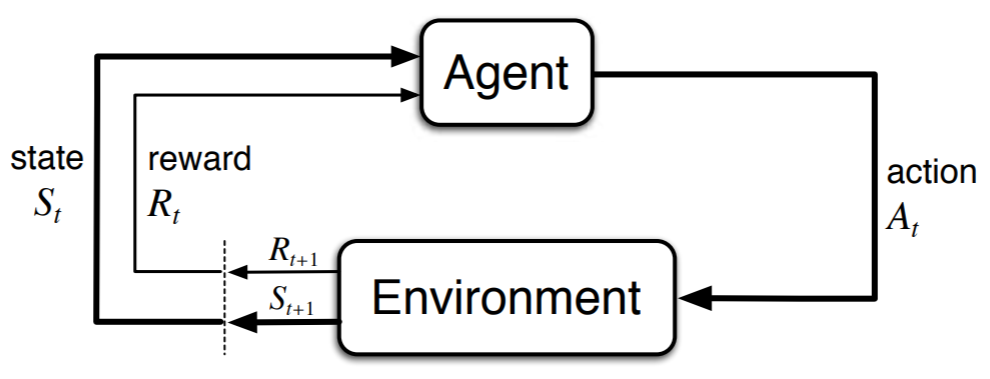
\includegraphics[width=0.6\textwidth]{pictures/RLInteractionSB}\\
    \caption[reinforcement learning cycle]{The cycle of agent-environment interaction as
        shown in ``Reinforcement learning: An introduction''\cite{suba18}}\label{fig:rl_cycle}
\end{figure}

\marginpar{sets and values}
The state $S_t$ is part of a set $S$ containing all possible environment states. Since its likely that not all actions are valid in each environment state the agents action selection is based on a restricted set $A_t\in A(S_t)$. In a multiagent environment however, every agent chooses its action and adds it into a joint action set, which is executed collectively on the environment \cite{buba10}. The reward $R_t$ is element of a set of possible rewards $R$, which is a subset of real numbers $R \subset \mathbb{R}$. Therefore, the reward can potentially be negative or very low to emphasize a bad action. The general concept of RL, as defined by Sutton and Barto, is to maximize rewards. Thus, unlike machine learning approaches the agent starts with no knowledge about good or bad actions and enhances the decision-making by aiming to improve the reward.

\marginpar{policy}
Sutton and Barto continue by defining the agents action selection with respect to the current state as a policy $\pi$. They explain further that a policy could be as simple as a lookup table, mapping states to actions or it could contain a complicated search process for the best decision. In most cases it is of stochastic nature, mapping actions and states with probabilities. During environment interactions agents gain rewards, which then can be used to update the policy accordingly. For example, should the reward be low or negative it could be interpreted as a penalty. In return the policy $\pi(a \mid s)$ could then be adapted to set a very low probability for that action in combination with that certain state. So next time the agent finds itself in that state the bad action is not very likely to be chosen again.

\marginpar{value function}
While rewards only rate the immediate situation, a value function, i.e. the state-value function $v_{\pi}(s)$ for a policy $\pi$ can be used to estimate the long-term value of a state $s$. The result is the total accumulated reward an agent could get down the line following that state and choosing actions based on the current policy. States that offer immediate high reward could end in
% The value function is of importance, due to states bringing high rewards could end in
low reward streaks. Or the opposite could be the case, where a low reward state could subsequently yield high rewards. Therefore, value functions are of great use to achieve the maximum reward.
% Other value functions can also take the executed
% action into account to reach the state from which the rewards are estimated.

\marginpar{exploration vs exploitation}
The last part to note about RL is that it entails the problem of balancing exploration and exploitation. In order to learn, an agent has to explore the options given. However, since maximizing rewards is the goal an agent could become greedy and exploit its knowledge by choosing actions of which it knows to result in small but positive rewards. If an agent doesn't explore enough the best action sequence will stay hidden and if an agent always explores without exploiting its knowledge, chances are that the reward will not be optimal.

\section{Proximal Policy Optimization}
TODO: introduce PPO as learning algorithm!

\marginpar{intro}
In 2017 Schulman et al. introduced the concept of Proximal Policy Optimization (PPO) in
the article ``Proximal Policy Optimization Algorithms''\cite{scwo17}.
This section is solely based on that article in order to explain the Algorithm.
Policy optimization is the improvement of the action selection strategy $\pi$ based on the
current state $s_{t}$. This is achieved by rotating two steps: 1. sampling data from the policy and 2.
optimizing that data through several epochs.

\marginpar{TRPO, Advantage func}
The origin of PPO lies in a similar approach called Trust Region Policy Optimization (TRPO).
TRPO strives to maximize the following function:
\begin{equation}\label{TRPO}
    \underset{\theta}{maximize}\,\hat{\mathbb{E}}_{t} [\frac{\pi_{\theta}(a_{t} \mid s_{t})}{\pi_{\theta_{old}}(a_{t} \mid s_{t})}
    \hat{A}_{t}-\beta \, KL[\pi_{\theta_{old}}(\cdot \mid s_{t}),\pi_{\theta}(\cdot \mid s_{t})]]
\end{equation}
with $\hat{A}_{t}$ as an estimator of the advantage function. The advantage function often calculated with the
state-value function $V(s)$, a reward $r$ and a discount coefficient $\lambda$ over a period of Time $t$
\begin{equation}\label{advantage}
    \hat{A}_{t} = -V(s_{t})+r_{t}+\lambda r_{t+1}+ \ldots + \lambda^{T-t+1} r_{T-1} + \lambda^{T-t} V(s_{T})
\end{equation}

The fraction in the Minuend of \eqref{TRPO} can be replaced by
$r(\theta)$ %= \frac{\pi_{\theta}(a_{t} \mid s_{t})}{\pi_{\theta_{old}}(a_{t} \mid s_{t})}$
and represents the probability ratio of an
action in the current policy in comparison to the old policy, with $\theta$ being a policy parameter.
The result of $r(\theta)$ is greater than
one, if an action is very probable in the current policy. Otherwise the outcome lies between zero and one.
Schulman et al. further describe that TRPO maximizes the "surrogate" objective
\begin{equation}\label{TRPO surrogate}
    L^{CPI}(\theta) = \hat{\mathbb{E}}_{t}[ \frac{\pi_{\theta}(a_{t} \mid s_{t})}{\pi_{\theta_{old}}(a_{t} \mid s_{t})} \hat{A}_{t}]
    = \hat{\mathbb{E}}_{t}[r(\theta)\hat{A}_{t}]
\end{equation}
However, maximized on its own without a penalty this results in a large outcome and leads to drastic
policy updates.

\marginpar{problem TRPO}
In order to stay in a trust region, as the name suggests, a penalty is subtracted from the
surrogate function \eqref{TRPO surrogate}.
The penalty is the Subtrahend of equation \eqref{TRPO} and contains the fixed coefficient $\beta$.
Regardless of the function details and outcome of $KL$, the coefficient $\beta$
is hard to choose, since different problems require different penalty degrees. Even in a single problem
it could be necessary to adapt the coefficient, due to changes within the setting.

\marginpar{PPO}
Therefore Schulman et al. introduced
\begin{equation}\label{PPO}
    L^{CLIP}(\theta) = \hat{\mathbb{E}}_{t}[\min(r(\theta)\hat{A}_{t},clip(r(\theta), 1-\epsilon, 1+\epsilon)\hat{A}_{t})]
\end{equation}
which is very similar to \eqref{TRPO} but does not require coefficients.
The first part of $\min$ contains $L^{CPI}$ \eqref{TRPO surrogate}.
The second part contains a $clip$ function which narrows the space of policy mutation with
the small hyperparameter $\epsilon$. After applying the clip function $r(\theta)$ lies between
$[1-\epsilon,1+\epsilon]$. Calculating the minimum of the clipped and unclipped probability ratio
produces the lower bound of the unclipped $r(\theta)$, preventing the policy to change drastically.
%[TODO ???]

\marginpar{PPO Algo}
PPO is defined by the following equation
\begin{equation}\label{PPO Algorithm}
    L_{t}^{CLIP+VF+S}(\theta) = \hat{\mathbb{E}}_{t}[L_{t}^{CLIP}(\theta) - c_{1}L_{t}^{VF}(\theta) + c_{2}S[\pi_{\theta}](s_{t})]
\end{equation}
with $c_{1}$ and $c_{2}$ as coefficients. The authors point out that the loss function \\
$L_{t}^{VF} = (V_{\theta}(s_{t})-V_{t}^{targ})^2$
combines the policy surrogate and the value function error term and is
necessary once a neural network shares parameters between policy and value function.
Finally an entropy bonus $S$ is added to ensure exploration.
Schulman et al. continues to show an example of an Algorithm using PPO, see Fig. \ref{fig:ppo_algo_code}.
$N$ detonates (parallel) actors collecting data in T timesteps in each Iteration.
Afterwards the policy is optimized in K epochs by computing the Loss function \eqref{PPO Algorithm} on the
corresponding $NT$ timesteps of data, using a minibatch.
\begin{figure}[hpbt]
    \centering
    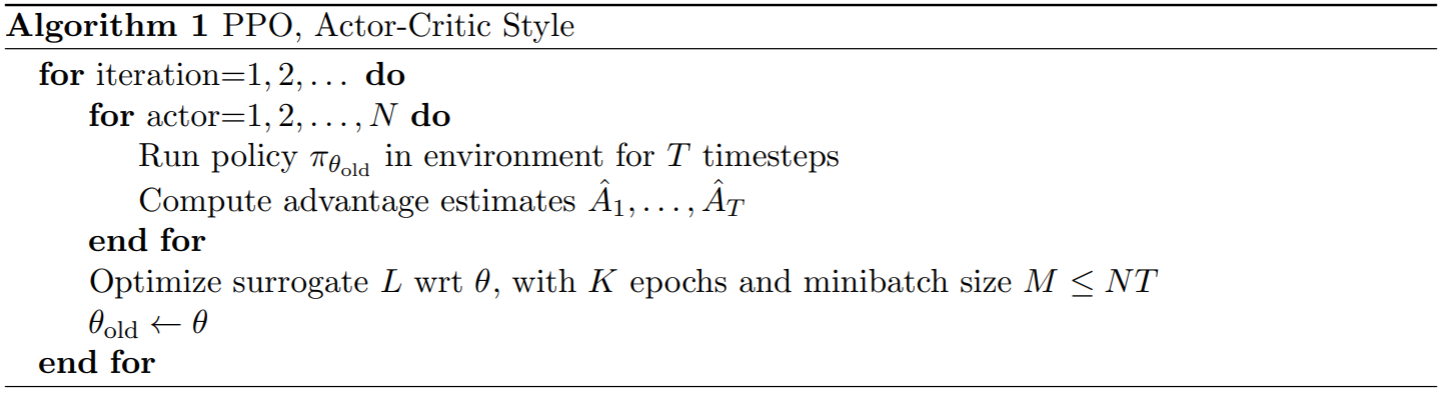
\includegraphics[width=1\textwidth]{pictures/ppo_algo_code.png}\\
    \caption[Exemplary use of PPO]{Exemplary use of PPO, as shown in ``Proximal Policy Optimization Algorithms''\cite{scwo17}}\label{fig:ppo_algo_code}
\end{figure}

\section{Deep Q-Learning}